\documentclass[english]{article}
\newcommand{\G}{\overline{C_{2k-1}}}
\usepackage[latin9]{inputenc}
\usepackage{amsmath}
\usepackage{amssymb}
\usepackage{lmodern}
\usepackage{mathtools}
\usepackage{enumitem}
%\usepackage{natbib}
%\bibliographystyle{plainnat}
%\setcitestyle{authoryear,open={(},close={)}}
\let\avec=\vec
\renewcommand\vec{\mathbf}
\renewcommand{\d}[1]{\ensuremath{\operatorname{d}\!{#1}}}
\newcommand{\pydx}[2]{\frac{\partial #1}{\partial #2}}
\newcommand{\dydx}[2]{\frac{\d #1}{\d #2}}
\newcommand{\ddx}[1]{\frac{\d{}}{\d{#1}}}
\newcommand{\hk}{\hat{K}}
\newcommand{\hl}{\hat{\lambda}}
\newcommand{\ol}{\overline{\lambda}}
\newcommand{\om}{\overline{\mu}}
\newcommand{\all}{\text{all }}
\newcommand{\valph}{\vec{\alpha}}
\newcommand{\vbet}{\vec{\beta}}
\newcommand{\vT}{\vec{T}}
\newcommand{\vN}{\vec{N}}
\newcommand{\vB}{\vec{B}}
\newcommand{\vX}{\vec{X}}
\newcommand{\vx}{\vec {x}}
\newcommand{\vn}{\vec{n}}
\newcommand{\vxs}{\vec {x}^*}
\newcommand{\vV}{\vec{V}}
\newcommand{\vTa}{\vec{T}_\alpha}
\newcommand{\vNa}{\vec{N}_\alpha}
\newcommand{\vBa}{\vec{B}_\alpha}
\newcommand{\vTb}{\vec{T}_\beta}
\newcommand{\vNb}{\vec{N}_\beta}
\newcommand{\vBb}{\vec{B}_\beta}
\newcommand{\bvT}{\bar{\vT}}
\newcommand{\ka}{\kappa_\alpha}
\newcommand{\ta}{\tau_\alpha}
\newcommand{\kb}{\kappa_\beta}
\newcommand{\tb}{\tau_\beta}
\newcommand{\hth}{\hat{\theta}}
\newcommand{\evat}[3]{\left. #1\right|_{#2}^{#3}}
\newcommand{\prompt}[1]{\begin{prompt*}
		#1
\end{prompt*}}
\newcommand{\vy}{\vec{y}}
\DeclareMathOperator{\sech}{sech}
\DeclarePairedDelimiter\abs{\lvert}{\rvert}%
\DeclarePairedDelimiter\norm{\lVert}{\rVert}%
\newcommand{\dis}[1]{\begin{align}
	#1
	\end{align}}
\newcommand{\LL}{\mathcal{L}}
\newcommand{\RR}{\mathbb{R}}
\newcommand{\NN}{\mathbb{N}}
\newcommand{\ZZ}{\mathbb{Z}}
\newcommand{\QQ}{\mathbb{Q}}
\newcommand{\Ss}{\mathcal{S}}
\newcommand{\BB}{\mathcal{B}}
\usepackage{graphicx}
% Swap the definition of \abs* and \norm*, so that \abs
% and \norm resizes the size of the brackets, and the 
% starred version does not.
%\makeatletter
%\let\oldabs\abs
%\def\abs{\@ifstar{\oldabs}{\oldabs*}}
%
%\let\oldnorm\norm
%\def\norm{\@ifstar{\oldnorm}{\oldnorm*}}
%\makeatother
\newenvironment{subproof}[1][\proofname]{%
	\renewcommand{\qedsymbol}{$\blacksquare$}%
	\begin{proof}[#1]%
	}{%
	\end{proof}%
}

\usepackage{centernot}
\usepackage{dirtytalk}
\usepackage{calc}
\newcommand{\prob}[1]{\setcounter{section}{#1-1}\section{}}


\newcommand{\prt}[1]{\setcounter{subsection}{#1-1}\subsection{}}
\newcommand{\pprt}[1]{{\textit{{#1}.)}}\newline}
\renewcommand\thesubsection{\alph{subsection}}
\usepackage[sl,bf,compact]{titlesec}
\titlelabel{\thetitle.)\quad}
\DeclarePairedDelimiter\floor{\lfloor}{\rfloor}
\makeatletter

\newcommand*\pFqskip{8mu}
\catcode`,\active
\newcommand*\pFq{\begingroup
	\catcode`\,\active
	\def ,{\mskip\pFqskip\relax}%
	\dopFq
}
\catcode`\,12
\def\dopFq#1#2#3#4#5{%
	{}_{#1}F_{#2}\biggl(\genfrac..{0pt}{}{#3}{#4}|#5\biggr
	)%
	\endgroup
}
\def\res{\mathop{Res}\limits}
% Symbols \wedge and \vee from mathabx
% \DeclareFontFamily{U}{matha}{\hyphenchar\font45}
% \DeclareFontShape{U}{matha}{m}{n}{
%       <5> <6> <7> <8> <9> <10> gen * matha
%       <10.95> matha10 <12> <14.4> <17.28> <20.74> <24.88> matha12
%       }{}
% \DeclareSymbolFont{matha}{U}{matha}{m}{n}
% \DeclareMathSymbol{\wedge}         {2}{matha}{"5E}
% \DeclareMathSymbol{\vee}           {2}{matha}{"5F}
% \makeatother

%\titlelabel{(\thesubsection)}
%\titlelabel{(\thesubsection)\quad}
\usepackage{listings}
\lstloadlanguages{[5.2]Mathematica}
\usepackage{babel}
\newcommand{\ffac}[2]{{(#1)}^{\underline{#2}}}
\usepackage{color}
\usepackage{amsthm}
\newtheorem{theorem}{Theorem}[section]
%\newtheorem*{theorem*}{Theorem}[section]
\newtheorem{conj}[theorem]{Conjecture}
\newtheorem{corollary}[theorem]{Corollary}
\newtheorem{example}[theorem]{Example}
\newtheorem{lemma}[theorem]{Lemma}
\newtheorem*{lemma*}{Lemma}
\newtheorem{problem}[theorem]{Problem}
\newtheorem{proposition}[theorem]{Proposition}
\newtheorem*{proposition*}{Proposition}
\newtheorem*{corollary*}{Corollary}
\newtheorem{fact}[theorem]{Fact}
\newtheorem*{prompt*}{Prompt}
\newtheorem*{claim*}{Claim}
\newcommand{\claim}[1]{\begin{claim*} #1\end{claim*}}
%organizing theorem environments by style--by the way, should we really have definitions (and notations I guess) in proposition style? it makes SO much of our text italicized, which is weird.
\theoremstyle{remark}
\newtheorem{remark}{Remark}[section]

\theoremstyle{definition}
\newtheorem{definition}[theorem]{Definition}
\newtheorem{notation}[theorem]{Notation}
\newtheorem*{notation*}{Notation}
%FINAL
\newcommand{\due}{25 September 2017} 
\RequirePackage{geometry}
\geometry{margin=.7in}
\usepackage{todonotes}
\title{MATH 8301 Homework III}
\author{David DeMark}
\date{\due}
\usepackage{fancyhdr}
\pagestyle{fancy}
\fancyhf{}
\rhead{David DeMark}
\chead{\due}
\lhead{MATH 8301}
\cfoot{\thepage}
% %%
%%
%%
%DRAFT

%\usepackage[left=1cm,right=4.5cm,top=2cm,bottom=1.5cm,marginparwidth=4cm]{geometry}
%\usepackage{todonotes}
% \title{MATH 8669 Homework 4-DRAFT}
% \usepackage{fancyhdr}
% \pagestyle{fancy}
% \fancyhf{}
% \rhead{David DeMark}
% \lhead{MATH 8669-Homework 4-DRAFT}
% \cfoot{\thepage}

%PROBLEM SPEFICIC

\newcommand{\lint}{\underline{\int}}
\newcommand{\uint}{\overline{\int}}
\newcommand{\hfi}{\hat{f}^{-1}}
\newcommand{\tfi}{\tilde{f}^{-1}}
\newcommand{\tsi}{\tilde{f}^{-1}}
\newcommand{\PP}{\mathcal{P}}
\newcommand{\nin}{\centernot\in}
\newcommand{\seq}[1]{({#1}_n)_{n\geq 1}}
\newcommand{\Tt}{\mathcal{T}}
\newcommand{\card}{\mathrm{card}}
\newcommand{\setc}[2]{\{ #1\::\:#2 \}}
\newcommand{\Fcal}{\mathcal{F}}
\newcommand{\cbal}{\overline{B}}
\newcommand{\Ccal}{\mathcal{C}}
\begin{document}
	\maketitle
	\section*{Notation}
	\begin{itemize}
		\item We let the topology of a topological space $X$ be denoted $\Tt(X)$ unless this is insufficient in context to avoid confusion.
		\item We let the cardinality of a set or topological space (interpreted as a set) $X$ be denoted $\abs{X}$.
		\item We let $S$ be a set and denote its power set as $\PP(S)$
		\item When it is understood that our context is some metric space $X$, we let the open ball of radius $\delta$ around $x\in X$ be denoted $B_\delta(x)$ and its closed counterpart be denoted $\overline B_\delta(x)$
	\end{itemize}
	\prob{1}Let $(V,\Fcal)$ be a simplicial complex and $\abs{(V,\Fcal)}$ its geometric realization.
	\begin{proposition*}
	 $\abs{(V,\Fcal)}$ is compact if and only if $\abs{V}<\infty$.
	\end{proposition*}
\begin{proof}
	$(\impliedby)$ We let $\abs{V}=m<\infty$. Then, as an individual $n$-simplex (where $n<m$) $\delta^n\subset \RR^{n+1}\subseteq \RR^m$ is closed under the standard topology of $\RR^{n+1}$, which is itself closed as a subset of $\RR^{m}$, we have that $\delta^n$ is closed under the standard topology of $\RR^{m}$. 
	Furthermore, we have that $\abs{\PP(V)}=2^{m}<\infty$, so as $\Fcal\subset \PP$, we have that $(V,\Fcal)$ is composed of the union of finitely many simplices. 
	Thus, $\abs{(V,\Fcal)}$ is a finite union of closed sets and hence is itself closed. 
	As $\abs{(V,\Fcal)}\subset \overline{B}_{1}(\vec{0})\subset \RR^m$, we have that $\abs{(V,\Fcal)}$ is a closed and bounded set and thus by Heine-Borel, is compact.
	
	$(\implies)$ We show the contrapositive, that is, if $\abs{V}=\infty$ then $\abs{(V,\Fcal)}$ is non-compact.
	 We show this by explicitly constructing an open cover with no finite subcover. For $v\in V$, we let $U_v=B_{\frac{1}{4}}(\vec{v})$ where $\vec{v}\in \abs{(V,\Fcal)}$ corresponds to $v\in V$. We then let $W=\abs{(V,\Fcal)}\setminus \left(\bigcup_{v\in V}\cbal_\frac{1}{8}(\vec v)\right)$.
	  We claim that $W$ is open under the topology of $\abs{(V,\Fcal)}$.
	   We consider the set $\tilde{W}=\RR^{\abs{V}}\setminus \left(\bigcup_{v\in V}\cbal_{\frac{1}{8}}(\vec{v})\right)$.
	    Then, as any finite-dimensional subspace of $\RR^{\abs{V}}$ must contain only finitely many of the vertex-realizations $\vec{v}$, any projection of $\tilde{W}$ to $\RR^d$ where $d$ is finite is simply the space $\RR^d$ with finitely many closed balls removed. 
	    Thus, $\tilde W$ is open, and as $W=\abs{(V,\Fcal)}\cap \tilde W$, we have that $W$ is indeed open.
	    Then, $\Ccal=\{U_v\}_{v\in V}\cup W$ is an open cover of $\abs{(V,\Fcal)}$ and as $\vec{v}$ is an element of only one set in $\Ccal$ for each $v\in V$, we have that no finite subcover could exist.
	     Hence, $\abs{(V,\Fcal)}$ is noncompact.
\end{proof}
	\prob{2}
	\begin{proposition*}
	$\abs{(V,\Fcal)}$ is connected if and only if for any two vertices $v,w\in V$, there exists a sequences of vertices $v=v_0,v_1,v_2,\hdots,v_m$ such that each of $e_m=\{v_{m-1},v_m\}\in \Fcal$ for $m=1,\hdots,n$. 
	\end{proposition*}

\begin{proof}
We first get one lemma out of the way, applying a theoretical sledgehammer to this hanging nail:
\begin{lemma}
Let $P$ be a smallest path in the graph theoretic sense (with no vertex repeats) between two vertices $v,w$ embedded in a (not necessarily finite) graph $G$. Then $P$ is finite.
\end{lemma}	
\begin{subproof}
	We construct the following ordering on $V(P)$: we let $v$ be the minimal element of $(V(P),\leq)$, and let $a\leq b$ if any path $P'\subset P$ between $v$ and $b$ must necessarily pass through $a$. We note that as each vertex besides $w$ has a unique successor, this is a well-ordering. We let $c(a)$ denote the cardinality of the minimal path $P_a\subset P$ from $v$ to $a$. We claim that $c(a)\in \NN$ for all $a\in V(P)$. We proceed by transfinite induction. Our claim holds trivially for $v$, as $c(v)=0$. We then suppose that our claim holds for $a\in P$ and note that for $b$ a successor to $a$, $c(b)\leq c(a)+1$ as any path of length $c(a)$ from $v$ to $a$ can be extended by one edge to be a path from $v$ to $b$. Finally, as only $v$ does not have a predecessor in $P$, $(P,\leq)$ contains no limit ordinals, so our proof by transfinite induction is complete. and there exists a finite path between $v$ and $w$. As $P$ is minimal by assumption, we now have that $P$ is finite.
\end{subproof}
Wow, that felt really dumb.

\textbf{\emph{Anyway}}, moving on, we have another lemma\textellipsis
\begin{lemma}
	Let $\Delta$ be the geometric realization of a single $n$-simplex  for any $n$. Then $\Delta$ is path-connected
\end{lemma}
\begin{subproof}
	We have that $\Delta=\{(t_1,\hdots,t_{n+1})\;:\; t_i\geq0\,\forall\: i \text{ and } \sum_{i=1}^n t_i=1\}$. We let $\vec{x}=(t_1,\hdots,t_{n+1}),\vec{y}=(s_1,\hdots,s_{n+1})\in \Delta$ be arbitrary, and let $\Phi:[0,1]\to \Delta$ be given by $\Phi(\tau)=(1-\tau)\vec{x}+\tau\vec{y}$. We have that for any $0\leq \tau_0\leq 1$, $x_0=(1-\tau_0)\vec{x} +\tau_0\vec{y}$ is, in each of its coordinates, a subtraction-free sum of non-negative numbers and is hence in the non-negative portion of $\RR^{n+1}$. Furthermore, we have that for $x_0=(j_1,\hdots,j_{n+1})$, $j_i=\tau_0 t_i +(1-\tau_0)s_i$. Thus, $\sum_{i=1}^n j_i=\tau_0\left(\sum_{i=1}^nt_i\right)+(1-\tau_0)\left(\sum_{i=1}^nt_i\right)=\tau_0(1)+(1-\tau_0)(1)=1$. Thus, $\Phi(\tau_0)\in \Delta$, is by construction a path-connection of $x,y$ and as a polynomial is obviously continuous.
\end{subproof}
By the above lemma, we now may restrict our attention to $(V,\Fcal')$ where $\Fcal'=\{S\in \Fcal\;:\; \card\:{S}\leq 2\}$, that is, the $1$-skeleton of $(V,\Fcal)$. 
%Indeed, note that if $\abs{(V,\Fcal')}$ is connected, then as any simplex of higher dimension contains its edges and is connected, we have that $\abs{(V,\Fcal)}$ is connected. Similarly, if $U$, $V$ is a disconnection of $\abs{(V,\Fcal')}$,   
We now attack the main theorem, this time assuming that $\abs{(V,\Fcal)}$ is a complex of $0$- and $1$-simplices.

$(\implies)$ We prove the contrapositive by contradiction: we assume that $\abs{(V,\Fcal)}$ is disconnected by $U,V$ but that for any two vertices, our path condition holds. We note that as $U,V$ nonempty and as edges are path-connected by the lemma, we have that for edge $e$ with $e\cap U\neq \emptyset$, we must have $\partial e=v_1,v_2\in U$ and similarly for $V$. Thus, we may assume there is a vertex $v\in U$ and $w\in V$ with a sequences of vertices $v_0,\hdots,v_m$ and edges $e_1,\hdots,e_m$ between them. We let $k=\max\{v_k\in U\}$. Then, $e_{k+1}\cap U\supset v_k$ and is hence nonempty. However, by maximality of $k$, we have that $v_{k+1}\in V$. Hence, $U\cap e_{k+1}$, $V\cap e_{k+1}$ is a disconnection of $e_{k+1}$, contradicting the lemma.

$(\impliedby)$ We again prove the contrapositive, this time directly. We suppose no path exists between vertices $v,w$. We let $V_1=\{a\in V\;:\; \exists \text{ path of edges between }v\text{ and }a\}$, and $V_2=V\setminus V_1$. We claim that all edges $e$ with one vertex of $V_1$ as a boundary component contain two vertices of $V_1$ as boundary components. Indeed, suppose $v'\in e\cap V_1$ and $v''=\partial e\setminus \{v'\}$, and let $P$ be an edge-path from $v$ to $v'$. Then, let $P'=P\cap e$. $P'$ is an edge-path from $v$ to $v''$, so $v''\in V_1$. Hence, as $\abs{(V,\Fcal)}$ is a complex of 1- and 0-simplices, we have that $\abs{(V_1,\Fcal_1)}$ is a maximally connected component of $\abs{(V,\Fcal)}$. We let $T$ be the union of the open tubular neighborhoods of radius $1/4$ about all edges in $\abs{(V_1,\Fcal_1)}$ and let $U=\RR^{\abs{V}+1}\setminus \overline{T}$. Then $U\cap\abs{(V,\Fcal)},T\cap \abs{(V,\Fcal)}$ is a disconnection of $\abs{(V,\Fcal)}$, completing our proof.   
\end{proof}
\prob{3}\textbf{\emph{The figures accompanying this problem may be found on the next page.}} \begin{proposition}
	The pairwise edge-identified hexagon with sides identified $abcab^{-1}c$ is homeomorphic to $N_2=\RR P^2\# \RR P^2=a_1^2a_2^2$, that is, the Klein Bottle.
\end{proposition}
\begin{proof}
	We first reorient $abcab^{-1}c=cabcab^{-1}$. We then make a cut $d$ at the head of $a$ and the tail of $b^{-1}$ to transform our hexagon into the triangble $cad$ and the pentagon $bcab^{-1}d^{-1}=ab^{-1}d^{-1}bc$ (Figure \ref{fig1}). We then reflect our triangle so that $cad=adc\mapsto c^{-1}d^{-1}a^{-1}$ and glue along $a$ to return the hexagon $c^{-1}d^{-1}b^{-1}d^{-1}bc$ (Figure \ref{fig2}). We then reorient to $cc^{-1}d^{-1}b^{-1}d^{-1}b$ and \say{close up the hole} at $c$ to return the square $d^{-1}b^{-1}d^{-1}b$ (Figure \ref{fig3}). This is well-known to be a representation of the Klein Bottle, but for completeness' sake, we reorient to $d^{-1}bd^{-1}b^{-1}$ and make another cut at the head of $b$ and the head of $d^{-1}$ (Figure \ref{fig3}) to yield the pair of triangles $d^{-1}e^{-1}b$ and $eb^{-1}d^{-1}$. We reflect the first of these such that $d^{-1}e^{-1}b\mapsto b^{-1}ed$ and reorient the second to $d^{-1}eb^{-1}$, then paste along $d$ to yield $eb^{-1}b^{-1}e$ (Figure \ref{fig4}). We rename by $b\mapsto a_1^{-1}$ and $e\mapsto a_2$ to relabel our square $a_2a_1^2a_2$ then reorient to finally yield $a_1^2a_2^2$. This completes our messy collage-making.
\end{proof}
\appendix
\begin{figure}[h]\centering
	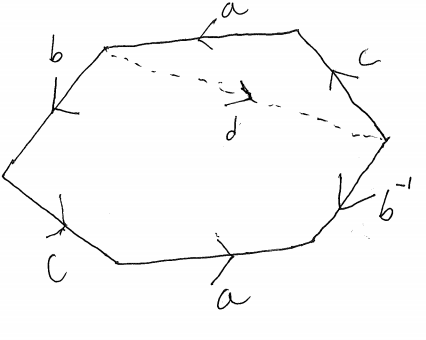
\includegraphics[scale=.6]{3-3fig1}\caption{The hexagon $abcab^{-1}c$, with the cut $d$ indicated \label{fig1}}
\end{figure}
\begin{figure}[h]\centering
	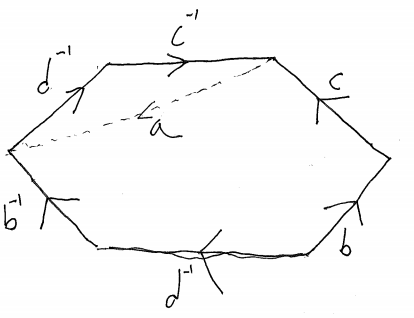
\includegraphics[scale=.6]{3-3fig2}\caption{The hexagon $c^{-1}d^{-1}b^{-1}d^{-1}bc$, with the gluing along $a$ indicated \label{fig2}}
\end{figure}
\begin{figure}[h]\centering
	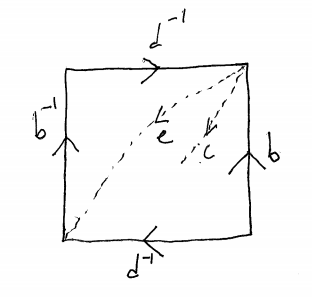
\includegraphics[scale=.6]{3-3fig3}\caption{The square $d^{-1}bd^{-1}b^{-1}$, with the gluing along $c$ and the to-be-made cut along $e$ indicated \label{fig3}}
\end{figure}
\begin{figure}[h]\centering
	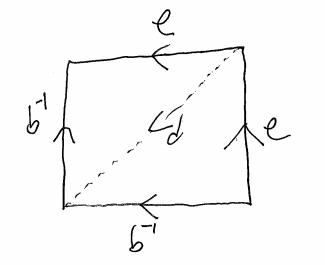
\includegraphics[scale=.6]{3-3fig4}\caption{The square $eb^{-1}b^{-1}e$, with the gluing along $d$ indicated \label{fig4}}
\end{figure}
\end{document}
